%%%%%%%%%%%%%%%%%%%%%%%%%%%%%%%%%%%%%%%%%
% Friggeri Resume/CV
% XeLaTeX Template
% Version 1.2 (3/5/15)
%
% This template has been downloaded from:
% http://www.LaTeXTemplates.com
%
% Original author:
% Adrien Friggeri (adrien@friggeri.net)
% https://github.com/afriggeri/CV
%
% License:
% CC BY-NC-SA 3.0 (http://creativecommons.org/licenses/by-nc-sa/3.0/)
%
% Important notes:
% This template needs to be compiled with XeLaTeX and the bibliography, if used,
% needs to be compiled with biber rather than bibtex.
%
%%%%%%%%%%%%%%%%%%%%%%%%%%%%%%%%%%%%%%%%%

\documentclass[]{scoggins-cv} % Add 'print' as an option into the square bracket to remove colors from this template for printing

\usepackage{fontspec}
\newfontfamily{\FA}[Path = fonts/]{fontawesome-webfont}

\usepackage{ragged2e}

\usepackage{marginnote}

\def\faEnvelope{{\FA\symbol{"F0E0}}}
\def\faGithub{{\FA\symbol{"F09B}}}
\def\faDesktop{{\FA\symbol{"F108}}}
\def\faPhone{{\FA\symbol{"F095}}}
\def\faHandPointerO{{\FA\symbol{"F25A}}}
\def\faMapMarker{{\FA\symbol{"F041}}}
\def\faVideoCamera{{\FA\symbol{"F03D}}}
\def\faCloudDownload{{\FA\symbol{"F0ED}}}

\input{citationskip}

\begin{document}

\header

%----------------------------------------------------------------------------------------
%	Contact
%----------------------------------------------------------------------------------------

\aside{Contact}{0.0325}{
    %
    \vspace*{-0.1cm}
    %
    \href{mailto:mts2188@columbia.edu}{{\addfontfeature{Color=linkblue}mts2188@columbia.edu}\ \faEnvelope}\\[0.5em]
    %
    \href{https://github.com/mscoggs}{{\addfontfeature{Color=linkblue}github.com/mscoggs}\ \faGithub}\\[0.5em]
    %
    \href{mscoggs.github.io}{{\addfontfeature{Color=linkblue}mscoggs.github.io}\ \faHandPointerO}\\[0.5em]
    %
    \href{tel:360-325-3398}{{\addfontfeature{Color=linkblue}+1 (360) 325 3398)}\ \faPhone}\\[0.5em]
    %
    \href{https://www.astro.columbia.edu/content/matthew-scoggins}{{\addfontfeature{Color=linkblue}\small Astronomy Department }\\
        \href{https://www.astro.columbia.edu/content/matthew-scoggins}{{\addfontfeature{Color=linkblue}\small Columbia University}}\ \faMapMarker}
    %
}

%----------------------------------------------------------------------------------------
%	EDUCATION
%----------------------------------------------------------------------------------------

\section{Education}

\begin{entrylist}

    %------------------------------------------------

    \entry
    {2021--}
    {PhD {\normalfont Astrophysics}}
    {Columbia University, New York, NY}
    {%
        \vspace{-1em}
        \begin{list}{{\color{numcolor}$-$}}{\cvlist}
            \item On connecting the 'direct-collapse' formation mechanism for suppermassive black holes to observation
            \item On extending the lifetime of habitable planets via star-lifting, a possible technosignature
            \item Advised by Zoltan Haiman, David Kipping
        \end{list}
    }

    %------------------------------------------------

    \entry
    {2015--2020}
    {BS {\normalfont Physics and Math,} BA {\normalfont Philosophy}}
    {Western Washington University, Bellingham WA}

    %------------------------------------------------

    \entry
    {2013-2015}
    {AS}
    {Whatcom Community College, Bellingham WA}

    %------------------------------------------------

\end{entrylist}

%----------------------------------------------------------------------------------------
%	ABOUT
%----------------------------------------------------------------------------------------

\aside{About Me}{0.035}{
    \footnotesize
    I am a first-year PhD Student in the Department of Astronomy at Columbia.
    My research interests span most areas of computational astrophysics and cosmology.
    Specifically, I'm interested in questions involving black holes, the early universe, and dark matter.
    Outside of academia I enjoy mountain climbing, skiing, videogames, piano, motorcycles, and chess.
}

%----------------------------------------------------------------------------------------
%	POSITIONS
%----------------------------------------------------------------------------------------

\section{Positions}

\begin{entrylist}

    %------------------------------------------------

    \entry
    {2021--}
    {Graduate Researcher}
    {Columbia University, New York, NY}
%    {%
%        \vspace{-1em}
%        \begin{list}{{\color{numcolor}$-$}}{\cvlist}
%            \item Work on statistical and computational data analysis problems
%                  \ifdefined \onepage \else
%                      applied to stellar and exoplanetary astronomy
%                  \fi
%            \item Develop algorithms and open-source software for timeseries analysis
%        \end{list}
%    }

  \entry
  {2021--}
  {Graduate Teaching Assistant}
  {Columbia University, New York, NY}
  {%
      \vspace{-1em}
      \begin{list}{{\color{numcolor}$-$}}{\cvlist}
        \item Spring 2022: Astrophysics II for Mary Putman
        \item Fall 2021: Another Earth for Caleb Scharf
      \end{list}
  }

    %------------------------------------------------
    \entry
    {2015--2021}
    {Undergraduate Researcher}
    {Western Washington University, Bellingham, WA}
    {%
        \vspace{-1em}
        \begin{list}{{\color{numcolor}$-$}}{\cvlist}
            \item Projects on machine learning applied to astronomy, flare cycles,
            quantum dynamics, and quantum foundations.
            \item Developed 2 open source simulators, \texttt{no\_wave\_qm} which simulates
            a no-wave approach to QM and \texttt{qubit\_simulation} which applies Monte-Carlo
            methods to find paths which optimally prepare a desired state.
        \end{list}
    }

\end{entrylist}

%----------------------------------------------------------------------------------------
%	STATS
%----------------------------------------------------------------------------------------

\aside{stats}{0.075}{
    \vspace*{0.5em}
    \input{pubs_summary}
}

%----------------------------------------------------------------------------------------
%	AWARDS
%----------------------------------------------------------------------------------------

\section{Honors \& Awards}

\begin{entrylist}

    \entry
    {2020}
    {Magna Cum Laude in both BS \& BA}
    {WWU, Bellingham, WA}
    {%
        \vspace*{-1.1em}
    }

    %------------------------------------------------
    \entry
    {2020}
    {Graduation w/ Merit in Mathematics}
    {WWU, Bellingham, WA}
    {%
        \vspace*{-1.1em}
    }
    %------------------------------------------------
    \entry
    {2019}
    {Material Science Undergraduate Research Grant}
    {WWU, Bellingham, WA}
    {%
        \vspace*{-1.1em}
    }

    %------------------------------------------------
    \entry
    {2018-2019}
    {Oscar Edwin Olson Scholarship (x2)} % Award
    {WWU, Bellingham, WA}
    {%
        \vspace*{-1.1em}
    }

    %------------------------------------------------
    \entry
    {2018}
    {Willard A. and Anne W. Brown Astronomy Scholarship} % Award
    {WWU, Bellingham, WA}
    {%
        \vspace*{-1.1em}
    }

    %------------------------------------------------
    \entry
    {2018}
    {Summer Student Research Stipend} % Award
    {WWU, Bellingham, WA}
    {%
        \vspace*{-1.1em}
    }

\end{entrylist}

%----------------------------------------------------------------------------------------
%	REFS
%----------------------------------------------------------------------------------------

\aside{References}{0.0325}{
    %\textbf{Kevin Covey}\\
    %{\footnotesize waiting@wwu.edu}\\[0.3em]
    %\textbf{Armin Rahmani}\\
    %{\footnotesize dhogg@flatironinstitute.org}\\[0.3em]
    %\textbf{rory barnes}\\
    %{\footnotesize rory@astro.washington.edu}
}

%----------------------------------------------------------------------------------------
%	METRICS
%----------------------------------------------------------------------------------------

\ifdefined \onepage \else
    \section{metrics}

    % SUPER HACKY
    \raisebox{-0.9\height}[0pt][0pt]{
        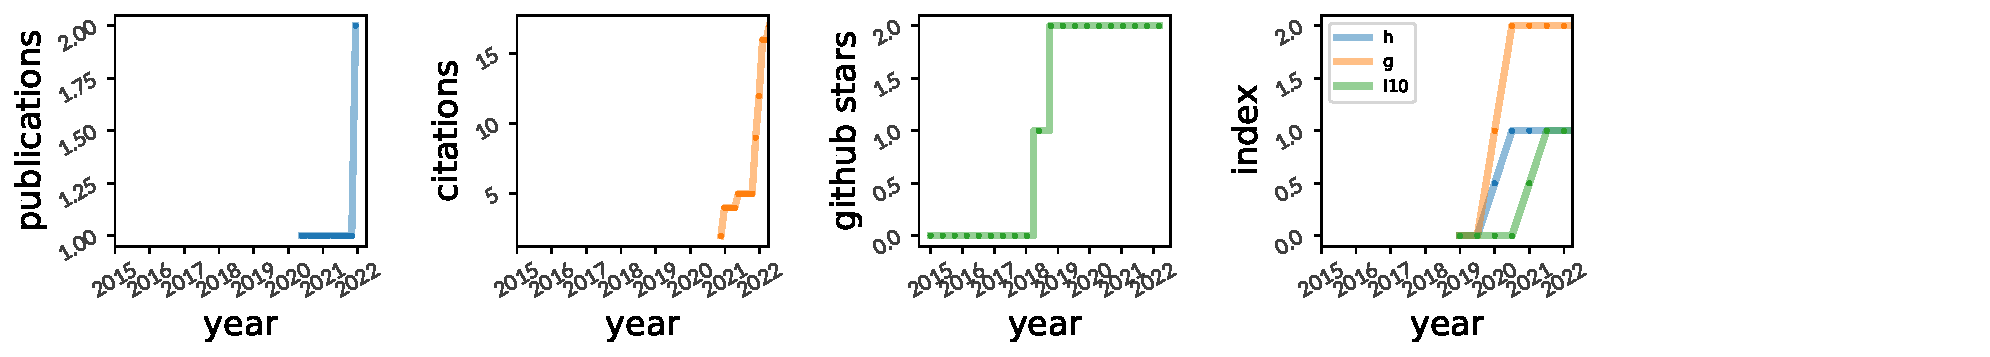
\includegraphics[height=1.25in]{metrics.pdf}
    }
    \pagebreak
\fi

%----------------------------------------------------------------------------------------
%	TEACHING
%----------------------------------------------------------------------------------------

%\ifdefined \onepage \else
%\aside{links}{0.05}{
%    {\color{numcolor}\faVideoCamera} \, \link{https://tinyurl.com/wnxmxb43}{LSST Lecture I}\\[0.5em]
%    {\color{numcolor}\faCloudDownload} \, \link{https://tinyurl.com/9247pj4}{LSST Worksheet I}\\[0.5em]
%    {\color{numcolor}\faVideoCamera} \, \link{https://drive.google.com/file/d/1PW-5Tkwnai7uQAZB4COFBUVTgWMZkE1P/view?usp=sharing}{LSST Lecture II}\\[0.5em]
%    {\color{numcolor}\faCloudDownload} \, \link{https://github.com/LSSTC-DSFP/LSSTC-DSFP-Sessions/tree/main/Session13/Day2}{LSST Worksheet II}\\[0.5em]
%}
%\fi
\section{Teaching \& Outreach}

\begin{entrylist}

    %------------------------------------------------

    \entry
    {2021-}
    {Graduate Teaching Assistant}
    {Columbia University}


    %------------------------------------------------

    \entry
    {2020-2021}
    {Mathematics Teaching Assistant}
    {WWU}

    %------------------------------------------------

    \entry
    {2017-2020}
    {Physics Teaching Assistant}
    {WWU}
    {%
        \vspace{-1em}
        \begin{list}{{\color{numcolor}$-$}}{\cvlist}
            \item Responsible for facilitating/grading a section of the weekly lab for Physics w/ Calc 161-163, 220, and Tools and Data Analysis 322
        \end{list}
    }

    %------------------------------------------------

    \entry
    {2018-2019}
    {Physics Study Group Facilitator}
    {WWU}
    {%
        \vspace{-1em}
        \begin{list}{{\color{numcolor}$-$}}{\cvlist}
            \item Responsible for creating content and leading a 2 hour weekly study group for Physics w/ Calc 161-163
        \end{list}
    }

    %------------------------------------------------

    \entry
    {2018-2019}
    {Math Tutoring Fellow}
    {WWU}
    {%
        \vspace{-1em}
        \begin{list}{{\color{numcolor}$-$}}{\cvlist}
            \item Responsible for tutoring a majority of the undergraduate math classes, Calculus I up to Intro. to Abstract Algebra.
        \end{list}
    }


\end{entrylist}

%----------------------------------------------------------------------------------------
%	STUDENTS
%----------------------------------------------------------------------------------------





  \section{Other}
      \begin{entrylist}

          %------------------------------------------------

          \entry
          {2019}
          {Student Faculty Hiring Committee}
          {WWU}


      \end{entrylist}
      %------------------------------------------------


    \aside{}{4.2}{
    {\footnotesize primary developer}\\[1em]
    \hrule
    {\footnotesize secondary developer}
    }
    \section{Software}

    \begin{entrylist}

        %------------------------------------------------

        \entry
        {\textbf{qubit\_sim}}
        {\textnormal{\url{github.com/mscoggs/qubit_simulation}}}
        {}
        {%
            \vspace{-1em}
            \begin{list}{{\color{numcolor}$-$}}{\cvlist}
                \item Simulating the evolution of a superconducting chip with the goal of finding patterns in the optimal protocols (values of the controls over time which evolve an initial state into a target state in the shortest possible time) over a variety of initial and target combinations.
            \end{list}
        }

        %------------------------------------------------

        \entry
        {\textbf{no\_wave\_qm}}
        {\textnormal{\url{github.com/mscoggs/no_wave_qm}}}
        {}
        {%
            \vspace{-1em}
            \begin{list}{{\color{numcolor}$-$}}{\cvlist}
                \item Simulating the evolution according to a hamilton-jacobi formulation of QM which replaces the wave with a configuration space density and equations of motion. Trajectory tracking using a 4-th order Runge Kutta technique.
            \end{list}
        }



    \end{entrylist}

    \section{Computing Experience}

    \begin{entrylist}

        %------------------------------------------------

        \entry
        {\textbf{Languages}(years): }
        {\textnormal{  \ C++(4), Python(4), C(3), Java(1), Matlab(1), Wolfram(1), Scheme(0.5), SQL(0.5)}}
        {}
        {
        }

        %------------------------------------------------
        \entry
        {\textbf{OS}: }
        {\textnormal{ \ Linux, mostly Ubuntu (5),  \   Windows (10+) \  Mac OS X (1)}}
        {}
        {
        }

        %------------------------------------------------
        \entry
        {\textbf{HPC Experience}: }
        {\textnormal{ WWU's CSCI Cluster \& CSE Cluster (Over 250 CPU years), Stampede2 (ongoing}}
        {}
        {
        }


    \end{entrylist}

%----------------------------------------------------------------------------------------
%	PUBLICATIONS
%----------------------------------------------------------------------------------------

\ifdefined \withpubs
    %
    \ifdefined \citationskip
    \else
        \def\citationskip{0.95}
    \fi
    %\aside{}{\citationskip}{
    %{\footnotesize citations $\longrightarrow$}\\[0em]
    %{\footnotesize (refereed in \textbf{bold})}
    %}
    %
    \section{Publications}
    %
    \begin{list}{}{\pubslist}
        \input{pubs}
    \end{list}
    %
    \vspace{1em}
\fi

%----------------------------------------------------------------------------------------
%	TALKS
%----------------------------------------------------------------------------------------


\ifdefined \withtalks

    \aside{}{0.95}{
        {\footnotesize {\color{numcolor}\faCloudDownload}\,: Downloadable}\\[0em]
        {\footnotesize {\color{numcolor}\faVideoCamera}\,: Watchable \phantom{XX.}}
    }
    \section{Selected Talks}
    %
    \begin{list}{}{\pubslist}
        \input{talks}
    \end{list}
\fi

\end{document}
